\documentclass[a4paper,12pt]{report}

\usepackage[english,greek]{babel}   % For Greek and English language
\usepackage{kmath,kerkis}           % Kerkis font
\usepackage{listings}               % For adding C++ code
\usepackage{xcolor}                 % For custom colors
\usepackage{graphicx}               % For including images
\usepackage{amsmath}                % For advanced math formatting
\usepackage{hyperref}               % For creating hyperlinks
\usepackage{geometry}               % To set page margins
\usepackage{subfig}                 % For subfigures
\usepackage{titlesec}               % For customizing chapter titles
\geometry{a4paper, margin=1in}      % Set page margins

\titleformat{\chapter}[block]
            {\normalfont\bfseries\huge}
            {\thechapter\quad}
            {0.5em}
            {}
            [\vspace{1ex}\noindent\rule{\textwidth}{0.4pt}]

\lstdefinestyle{verilog}{
    language=Verilog,
    basicstyle=\ttfamily\small,                     % Use small monospaced font
    keywordstyle=\color{blue},                      % Blue for keywords
    commentstyle=\color{green},                     % Green for comments
    stringstyle=\color{red},                        % Red for strings
    morekeywords={module,endmodule,always,if,else}, % Additional Verilog keywords
    backgroundcolor=\color{lightgray},              % Background color for code block
    showstringspaces=false,                         % Don't show space in strings
    frame=single,                                   % Frame around the code
    captionpos=b,                                   % Position of caption (bottom)
    breaklines=true,                                % Automatically break long lines
    breakatwhitespace=true,                         % Break lines at whitespace
}

\AtBeginEnvironment{lstlisting}{\selectlanguage{english}}
\AtEndEnvironment{lstlisting}{\selectlanguage{greek}}

\def\tl{\textlatin}
\def\tg{\textgreek}

\begin{document}

\title{\textbf{Ψηφιακά Συστήματα \tl{Hardware} σε Υψηλά Επίπεδα Λογικής 1} \\ Αναφορά Εργασίας}
\author{\textbf{Σάββας Τζανέτης} \\
\textbf{10889} \\
\href{mailto:empty@auth.gr}{\tl{stzanetis@ece.auth.gr}}}
\maketitle

\chapter*{Εισαγωγή}
    \large Αυτή η αναφορά είναι μέρος της εργασίας του μαθήματος \textbf{Ψηφιακά Συστήματα \tl{Hardware} σε Χαμηλά Επίπεδα Λογικής 1} του \textbf{Αριστοτέλιου πανεπιστημίου Θεσσαλονίκης}. \\
    Σε αυτή την εργασία, μας ζητήθηκε να υλοποιήσουμε μια αριθμομηχανή, καθώς και έναν επεξεργαστή \textbf{\tl{RISC-V}} με την βοήθεια των παρακάτω ασκήσεων σε γλώσσα \textbf{\tl{Verilog}}. \\
    Στην αναφορά θα γίνει μια σύντομη επεξήγηση των ασκήσεων, σχολιασμός του κώδικα και παρουσίαση των ζητούμενων διαγραμμάτων και κυματομορφών των προσομοιώσεων.
\chapter{Πρώτη Άσκηση}
    \large Στη πρώτη άσκηση μας ζητήθηκε να υλοποιήσουμε μια "Αριθμητική και Λογική Μονάδα" \textbf{\tl{(ALU)}}. \\ \\
    Η υλοποίηση μιας \textbf{\tl{ALU}} σε \textbf{\tl{Verilog}} είναι αρκετά απλή, καθώς αποτελείται από έναν \textbf{\tl{multiplexer}} που υλοποιήθηκε κάνοντας \tl{assign} στην έξοδο \tl{result} το ανάλογο αποτέλεσμα μετά από σύγκριση των παραμέτρων που έχουν οριστεί στην αρχή του κωδικά με τις διάφορες λειτουργίες που θέλουμε να εκτελεί η \tl{ALU}. Η σύγκριση γίνεται με την χρίση λογικόν πράξεων που προσομοιωνόσουν μια σειρά από \tl{else if} εντολές. Στη συνεχεία μετά από την επιλογή της ανάλογης λειτουργίας πραγματοποιείται η κατάλληλη πράξη μεταξύ των εισόδων \textbf{\tl{op1}} και \textbf{\tl{op2}}. Να σημειωθεί επίσης, πως στις ειδικές περιπτώσεις των πράξεων "\textbf{\tl{less than}}" και "\textbf{\tl{arithmetic shift right}}" οι είσοδοι \textbf{\tl{op1}} και \textbf{\tl{op2}} μετατρέπονται σε προσημασμένες τιμές για την σωστή λειτουργία των πράξεων.
    \vspace{1cm}
    \begin{lstlisting}[style=verilog]
assign result = (alu_op == ALUOP_AND) ? (op1 & op2):
    (alu_op == ALUOP_OR)          ? (op1 | op2)
    (alu_op == ALUOP_ADD)         ? (op1 + op2):
    (alu_op == ALUOP_SUB)         ? (op1 - op2):
    (alu_op == ALUOP_LTHAN)       ? ($signed(op1) < $signed(op2)):
    (alu_op == ALUOP_LSHIFTR)     ? (op1 >> op2[4:0]):
    (alu_op == ALUOP_LSHIFTL)     ? (op1 << op2[4:0]):
    (alu_op == ALUOP_ASHIFTR)     ? ($signed(op1) >>> op2[4:0]):
    (alu_op == ALUOP_XOR)         ? (op1 ^ op2):
    32'b0;  
    \end{lstlisting}
\chapter{Δεύτερη Άσκηση}
    \large Η δεύτερη άσκηση έχει ως ζητούμενο, την υλοποίηση της αριθμομηχανής με την βοήθεια του \textbf{\tl{alu.v}} \tl{module} της πρώτης άσκησης, αλλά και ενός \\\textbf{\tl{testbench}} για την επαλήθευση της σωστής λειτουργίας της αριθμομηχανής. Για την μοντελοποίηση της αριθμομηχανής μας ζητήθηκαν δυο αρχεία, το αρχείο \textbf{\tl{calc.v}} το οποίο άφορα την γενική λειτουργιά της αριθμομηχανής, και το αρχείο \textbf{\tl{calc\_enc.v}} το οποίο είναι υπεύθυνο για την παράγωγη του ανάλογου σήματος \textbf{\tl{alu\_op}} το οποίο θα εισαχθεί στο \\\textbf{\tl{ALU}} \tl{module} της πρώτης άσκησης. \\ \\
    Ο κωδικοποιητής \textbf{\tl{calc\_enc.v}}, παράγει το κατάλληλο σήμα με την χρήση \textbf{\tl{Structural Verilog}}, ακολουθώντας τα σχήματα 2 έως 5 της εκφώνησης της εργασίας για την δημιουργία των κατάλληλων συνδυαστικών κυκλωμάτων. \\Η κωδικοποίηση αυτών των σημάτων γίνεται με την εισαγωγή τριών σημάτων εισόδου, τα οποία λειτουργούν ως ‘κουμπιά’ και τα ονομάζουμε \textbf{\tl{btnc}}, \textbf{\tl{btnl}} και \textbf{\tl{btnr}}. \\ \\
    Στο αρχείο \textbf{\tl{calc.v}} δημιουργούμε την βασική λειτουργιά της αριθμομηχανής συμφωνά με το Σχήμα 2.1 της εκφώνησης. Συγκεκριμένα:
    \begin{itemize}
        \item Υλοποιείται ο συσσωρευτής με την χρήση ενός \tl{always block}.
            \vspace{0.5cm}
            \begin{lstlisting}[style=verilog]
always @(posedge clk) begin
    if(btnu)
        accumulator <= 16'b0;
    else if(btnd)
        accumulator <= alu_out[15:0];
end 
            \end{lstlisting}
        \newpage
        \item Ή επέκταση πρόσημου.
            \vspace{0.5cm}
            \begin{lstlisting}[style=verilog]
wire[31:0] op1_extended = {{16{accumulator[15]}}, accumulator};
wire[31:0] op2_extended = {{16{sw[15]}}, sw};
            \end{lstlisting}
        \item Συνδέεται η \tl{ALU} που έχουμε ήδη υλοποιήσει.
            \vspace{0.5cm}
            \begin{lstlisting}[style=verilog]
alu my_alu (
    .op1(op1_extended),
    .op2(op2_extended),
    .alu_op(alu_op),
    .result(alu_out),
    .zero(zero)
); 
            \end{lstlisting}
        \item Το σύστημα έλεγχου της \tl{ALU}, δηλαδή το \tl{calc\_enc} module.
            \vspace{0.5cm}
            \begin{lstlisting}[style=verilog]
calc_enc encoder (
    .btnc(btnc),
    .btnl(btnl),
    .btnr(btnr),
    .alu_op(alu_op)
);
            \end{lstlisting}
    \end{itemize}
    \begin{figure}[h!]
        \centering
        \fbox{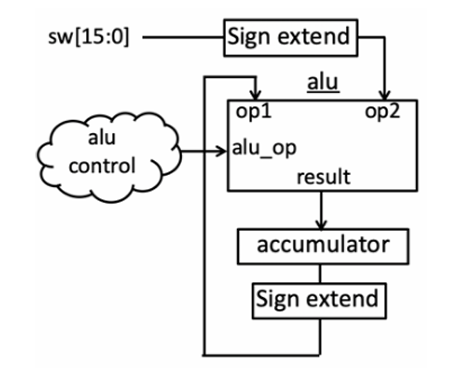
\includegraphics[width=0.65\textwidth]{21.png}}
        \caption{}
    \end{figure}
    \newpage
    Το \textbf{\tl{calc\_tb}} έχει έναν πολύ σημαντικό σκοπό. Με την βοήθεια αυτού του \textbf{\tl{testbench}} αρχείου γίνεται ο έλεγχος των παραπάνω υλοποιήσεων. Η εκφώνηση μας ζητάει να πραγματοποιήσουμε κάποια συγκεκριμένα \tl{test}, εκτελώντας συγκεκριμένες πράξεις με συγκεκριμένες τιμές ώστε να μπορέσουμε να συγκρίνουμε αργότερα τα αποτελέσματα με αυτά που μας έχουν δοθεί από την εκφώνηση. Τα αποτελέσματα αυτών των \tl{test} είναι:
    \vspace{0.5cm}
    \begin{lstlisting}[style=verilog]
# Reset: LED = 0000 (Expected: 0x0)
# ADD: LED = 354a (Expected: 0x354A)
# SUB: LED = 2316 (Expected: 0x2316)
# OR: LED = 3317 (Expected: 0x3317)
# AND: LED = 3010 (Expected: 0x3010)
# XOR: LED = 2fb2 (Expected: 0x2FB2)
# ADD: LED = 9a54 (Expected: 0x9A54)
# LogicalShiftLeft: LED = a540 (Expected: 0xA540)
# ShiftRight Arithmetic: LED = d2a0 (Expected: 0xD2A0)
# LessThan: LED = 0001 (Expected: 0x0001)
    \end{lstlisting}
    \vspace{0.5cm}
    Ενώ οι κυματομορφες που παράγονται από την προσομοίωση εμφανίζονται παρακάτω.
    \vspace{0.5cm}
    \begin{figure}[h!]
        \centering
        \fbox{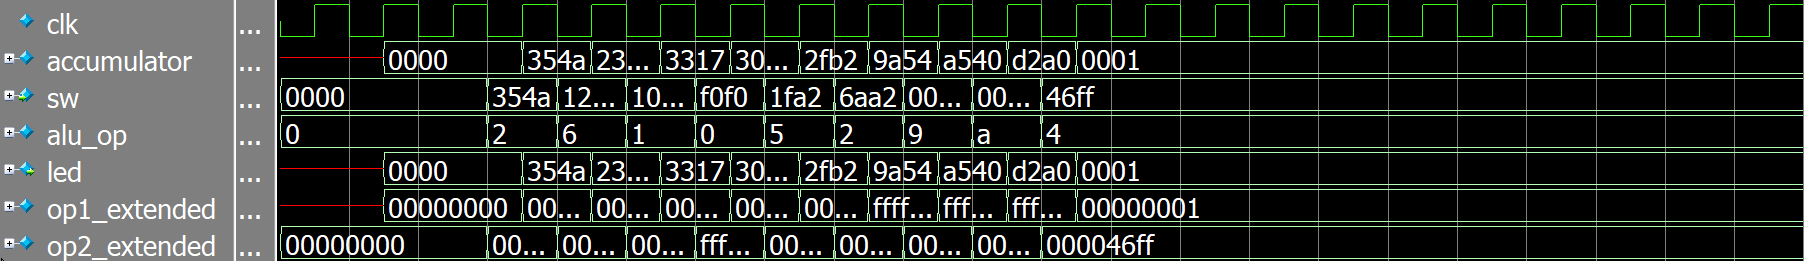
\includegraphics[width=1\textwidth]{22.png}}
        \caption{}
    \end{figure}
\chapter{Τρίτη Άσκηση}
    \large Σε αυτή την άσκηση της εργασίας, πρέπει να υλοποιήσουμε ένα \textbf{αρχείο καταχωρητών}, το οποίο θα είναι υπεύθυνο για την αποθήκευση των τιμών των καταχωρητών που θα χρησιμοποιούνται από τον \textbf{\tl{RISC-V}} επεξεργαστή μας.\\ \\
    Στην την υλοποίηση του αυτού του \tl{module}, η πρώτη διεργασία είναι η αρχικοποίηση των καταχωρητών με την τιμή μηδέν, εξασφαλίζοντας μια γνωστή αρχική κατάσταση. Η λειτουργία εγγραφής συγχρονίζεται με το σήμα ρολογιού και τα δεδομένα εγγράφονται στον καθορισμένο καταχωρητή εάν το σήμα εγγραφής είναι ενεργό και η διεύθυνση του καταχωρητή δεν είναι μηδέν. Επίσης, στην υλοποίηση χρησιμοποιήθηκαν \textbf{\tl{Non-Blocking}} εντολές, αποτρέποντας την εσφαλμένη χρίση των καταχωρητών με την καταγραφή λανθασμένων τιμών στην περίπτωση που χρησιμοποιηθεί η ίδια διεύθυνση για εγγραφή και ανάγνωση.
\chapter{Τέταρτη Άσκηση}
    \large Στόχος της άσκησης 4 είναι να σχεδιάσουμε ένα \textbf{\tl{datapath}} \tl{module}, μια μονάδα διαδρομής δεδομένων. Η μονάδα αυτί, μαζί με το \tl{module} της επόμενης άσκησης, καθώς και τη μνήμη εντολών και δεδομένων που μας δίνονται έτοιμες, θα ολοκληρώσουν την λειτουργιά του \textbf{\tl{RISC-V}} επεξεργαστή που θέλουμε να υλοποιήσουμε. \\ \\
    Η άσκηση αυτή, χωρίζεται σε πέντε τμήματα όπως θα δούμε και στο παρακάτω διάγραμμα. Πιο συγκεκριμένα τα τμήματα αυτά είναι:
     \begin{itemize}
        \item Το \tl{Program Counter (PC)}
            \vspace{0.5cm}
            \begin{lstlisting}[style=verilog]
always @(posedge clk) begin 
    if(rst)
        PC <= INITIAL_PC;
    else if(loadPC) begin 
        if(PCSrc)
            PC <= sum_pc_i;
        else
            PC <= PC + 4;
    end
end
            \end{lstlisting}
        \item Το \tl{Register File} που θα πρέπει να αρχικοποιήσουμε.
            \vspace{0.5cm}
            \begin{lstlisting}[style=verilog]
regfile my_regfile (
    .clk(clk),
    .write(RegWrite),
    .readReg1(instr[19:15]),
    .readReg2(instr[24:20]),
    .writeReg(instr[11:7]),
    .writeData(write_back_data),
    .readData1(alu_op1),
    .readData2(alu_op2)
);
            \end{lstlisting}
        \item \tl{Immediate Generation}.
            \vspace{0.5cm}
            \begin{lstlisting}[style=verilog]
assign input_i_addi = instr[31:20];
assign output_i_addi = {{20{input_i_addi[11]}}, input_i_addi};
assign input_i_sw = {instr[31:25], instr[11:7]};
assign output_i_sw = {{20{input_i_sw[11]}}, input_i_sw};
assign input_i_beq = {instr[31], instr[7], instr[30:25], instr[11:8]};
assign output_i_beq = {{19{input_i_beq[11]}}, input_i_beq, 1'b0};
            \end{lstlisting}
        \item Το \tl{ALU} που έχουμε υλοποιήσει στη πρώτη άσκηση και θα πρέπει να αρχικοποιήσουμε.
            \vspace{0.5cm}
            \begin{lstlisting}[style=verilog]
alu my_alu (
	.op1(alu_op1),
    .op2(mux_result_op2),
    .alu_op(ALUCtrl),
    .result(alu_result),
	.zero(Zero)
);
            \end{lstlisting}
        \item Το \tl{Branch Target}.
            \begin{lstlisting}[style=verilog]
assign left_add = output_i_beq << 1;
assign sum_pc_i = left_add + PC;
            \end{lstlisting}
        \item \tl{Write Back}.
            \begin{lstlisting}[style=verilog]
assign write_back_data = MemToReg ? dReadData : alu_result;
            \end{lstlisting}
    \end{itemize}
    \newpage
    Επιπλέον, αξίζει να σημειωθεί πως σε αρκετές περιπτώσεις, για την δημιουργία πολυπλεκτών, χρησιμοποιήσαμε εντολές \tl{assign} αντί ενός \tl{always block}. Αυτό έγινε για λόγους απλοποίησης, αλλά και για την αποτροπή σφαλμάτων λόγω καθυστερήσεων με την χρήση \tl{always block}.
    \vspace{0.5 cm}
    \begin{figure}[h!]
        \centering
        \fbox{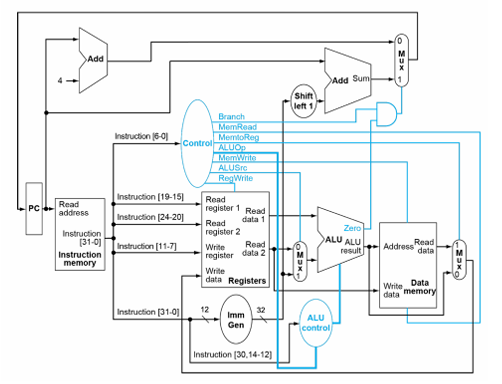
\includegraphics[width=0.85\textwidth]{41.png}}
        \caption{}
    \end{figure}
\chapter{Πέμπτη Άσκηση}
    \large Στην πέμπτη και τελευταία άσκηση, θα υλοποιήσουμε το τελευταίο στοιχείο του επεξεργαστή μας, την μονάδα έλεγχου, καθώς και θα υλοποιήσουμε ένα testbench για τον έλεγχο των λειτουργιών του. Θα δημιουργήσουμε δυο αρχεία, το \textbf{\tl{top\_proc.v}} και το \textbf{\tl{top\_proc\_tb.v}}. \\ \\
    Για το αρχειο \textbf{\tl{top\_proc.v}}, έπρεπε και πάλι να υλοποιήσουμε 7 τμήματα. Το πιο σημαντικό από αυτά όμως ήταν η υλοποίηση ενός \textbf{\tl{FSM (Finite State Machine)}}, για το οποίο έπρεπε να υλοποιήσουμε 3 \tl{Procedural Blocks}. Την Αποθήκευση κατάστασης, την επόμενη κατάσταση και τέλος την κατάσταση εξόδου. Τα 3 αυτά \tl{block} υλοποιήθηκαν χρησιμοποιώντας διάφορα \tl{always block}, δημιουργώντας ουσιαστικά διάφορους πολυπλέκτες για κάθε μια από τις πιθανές εντολές της εισόδου \textbf{\tl{instr}}.\\ \\
    Στο \textbf{\tl{testbench}} μας, συνδέουμε τα αρχεία \textbf{\tl{rom.v}} και \textbf{\tl{ram.v}} τα οποία μας έχουν δοθεί και δημιουργούμε ένα ρολόι για την εκτέλεση των απαραίτητων προσομοιώσεων. Στο αρχείο \textbf{\tl{rom\_bytes.data}} βρίσκονται οι εντολές \textbf{\tl{32-bit}} που θα πρέπει να 
    εκτελέσει ο επεξεργαστής για να επαληθεύει η\\
    \begin{figure}[h!]
        \centering
        \fbox{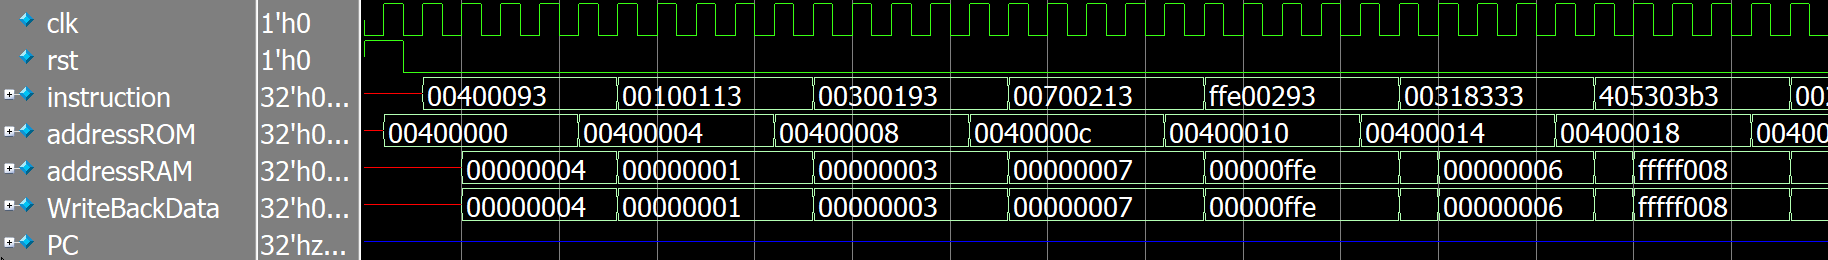
\includegraphics[width=1\textwidth]{51.png}}
        \caption{}
    \end{figure}
    ορθή λειτουργία του.
    
    Οι παραπάνω κυματομορφες αποτελούν ένα μικρό κομμάτι των κυματομορφών που παράχθηκαν από την προσομοίωση για λόγους διευκόλυνσης.
    
\end{document}